%% LaTeX-Beamer template for KIT design
%% by Erik Burger, Christian Hammer
%% title picture by Klaus Krogmann
%%
%% version 2.1
%%
%% mostly compatible to KIT corporate design v2.0
%% http://intranet.kit.edu/gestaltungsrichtlinien.php
%%
%% Problems, bugs and comments to
%% burger@kit.edu

\documentclass[18pt]{beamer}

%% SLIDE FORMAT

% use 'beamerthemekit' for standard 4:3 ratio
% for widescreen slides (16:9), use 'beamerthemekitwide'

\usepackage{templates/beamerthemekit}
% \usepackage{templates/beamerthemekitwide}

%% TITLE PICTURE

% if a custom picture is to be used on the title page, copy it into the 'logos'
% directory, in the line below, replace 'mypicture' with the 
% filename (without extension) and uncomment the following line
% (picture proportions: 63 : 20 for standard, 169 : 40 for wide
% *.eps format if you use latex+dvips+ps2pdf, 
% *.jpg/*.png/*.pdf if you use pdflatex)

%\titleimage{mypicture}

%% TITLE LOGO

% for a custom logo on the front page, copy your file into the 'logos'
% directory, insert the filename in the line below and uncomment it

%\titlelogo{mylogo}

% (*.eps format if you use latex+dvips+ps2pdf,
% *.jpg/*.png/*.pdf if you use pdflatex)

%% TikZ INTEGRATION

% use these packages for PCM symbols and UML classes
% \usepackage{templates/tikzkit}
% \usepackage{templates/tikzuml}

% the presentation starts here
\usepackage{templates/beamerthemekit}
% \usepackage{templates/beamerthemekitwide}
\usepackage{graphicx}
\usepackage{listings}
\usepackage{color}
\usepackage{textcomp}
\definecolor{listinggray}{gray}{0.9}
\definecolor{lbcolor}{rgb}{0.9,0.9,0.9}
\lstset{
	language=Java,
	backgroundcolor=\color{lbcolor},
	tabsize=4,
	rulecolor=,
        basicstyle=\footnotesize,
        aboveskip=5pt,
        upquote=true,
        columns=fixed,
        showstringspaces=false,
        extendedchars=true,
        breaklines=true,
        frame=single,
        showtabs=false,
        showspaces=false,
        showstringspaces=false,
        identifierstyle=\ttfamily,
        keywordstyle=\color[rgb]{0,0,1},
        commentstyle=\color[rgb]{0.133,0.545,0.133},
        stringstyle=\color[rgb]{0.627,0.126,0.941},
}
\usepackage[utf8]{inputenc}


\title[Prog Tut Nr. 2]{Tutorium Programmieren}
\subtitle{Tut Nr.2: Objekte und Methoden}
\author{Michael Friedrich}
\date{5. / 7.11.2013}
\institute{Institut f\"ur theoretische Informatik}
% Bibliography

\usepackage[citestyle=authoryear,bibstyle=numeric,hyperref,backend=biber]{biblatex}
\addbibresource{templates/example.bib}
\bibhang1em

\begin{document}

% change the following line to "ngerman" for German style date and logos
\selectlanguage{ngerman}

%title page
\begin{frame}
	\titlepage
\end{frame}

%table of contents
\begin{frame}{Outline/Gliederung}
	\tableofcontents
\end{frame}


\section{Variablen}

\begin{frame}[fragile]{Variablen}
\begin{block}{Was ist eine Variable?}
Eine Variable ist ein Bezeichner ($\equiv$ Name) für einen Speicherplatz im Rechner.
\end{block}
\pause
\begin{exampleblock}{Variablen in Java - Beispiel:}
	\begin{lstlisting}
	int meineZahl;			//Deklariert eine int - Variable
	meineZahl = 16;			//setzt sie auf die Zahl 16
	boolean istWahr = true;	//Deklariert eine boolean - Variable 
							//und weist ihr sofort einen Wert zu
	meineZahl = 42;			//aendert den Wert von 'meineZahl'
	\end{lstlisting}
	\end{exampleblock}
\end{frame}

\begin{frame}{Variablen}
\begin{block}{Variablen in Java - Allgemein:}
\begin{itemize}
	\item \textbf{Deklaration} - Namen \& Typ festlegen:\\
	\textit{Typ Variablenname;}
	\item \textbf{Initialisierung} - erstmalige Zuweisung eines Werts:\\
	\textit{Variablenname} = \textit{Wert;}\\
	\begin{itemize}
		\item gleichzeitige Deklaration \& Initialisierung:\\
		\textit{Typ Variablenname} = \textit{Wert;}
	\end{itemize}
	\item \textbf{Zuweisung} - Setzen eines Wertes:\\
	\textit{Variablenname} = \textit{Wert}
\end{itemize}
\end{block}
\pause
\textbf{Attribute} sind Variablen auf Klassenebene.
\end{frame}

\begin{frame}{Die elementaren Datentypen in Java}
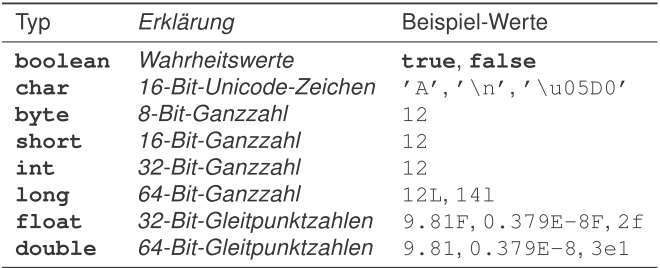
\includegraphics[width=\linewidth]{logos/datentypen}
\end{frame}

\begin{frame}{Wertebereiche der elementaren Datentypen}
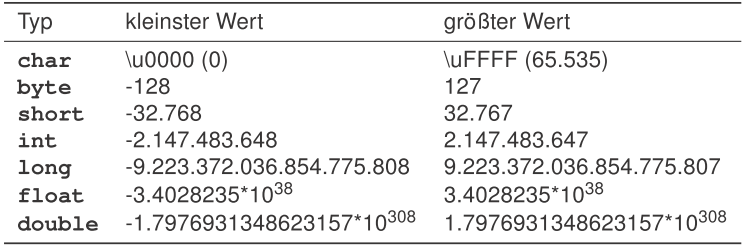
\includegraphics[width=\linewidth]{logos/werte}
\end{frame}


\subsection{Variablenoperationen}
\begin{frame}{Variablenoperationen}
\begin{block}{(die wichtigsten) Operationen mit Zahlen}
\begin{itemize}
	\item \textbf{x + y, x - y, x * y, x / y}: (fast) wie aus der Mathematik bekannt
	\item \textbf{x \% y}: Modulo (Rest der Division von x und y)
\end{itemize}
$\rightarrow$ liefern wieder Zahlen zurück
\pause
\begin{itemize}
	\item \textbf{x == y, x != y}: Gleichheit, Ungleichheit
	\item \textbf{x $>$ y, x $<$ y, x $>=$ y, x $<=$ y}: größer/kleiner (gleich)\\
\end{itemize}
$\rightarrow$ liefern boolesche Werte (true oder false) zurück
\end{block}
\pause
\begin{block}{Konkatenation von Zeichenketten}
\begin{itemize}
\item \textbf{\textit{string1} + \textit{string2}} hängt beide Strings aneinander
\end{itemize}
$\rightarrow$ liefert wieder einen String zurück
\end{block}
\end{frame}

\begin{frame}{Variablenoperationen}
\begin{block}{Operationen mit Wahrheitswerten}
\begin{itemize}
	\item \textbf{!a} : NOT
	\item  \textbf{a \&\& b}: logisches AND
	\item \textbf{a $||$ b}: logisches OR
	\item \textbf{a \^{} b}: XOR (exklusives OR)\\
	$\rightarrow$ liefern wieder boolesche Werte zurück
\end{itemize}
\end{block}
\end{frame}

\begin{frame}[fragile]{Variablenoperationen}
\begin{alertblock}{Vorsicht bei der Division!}
Die Division zweier Ganzzahlen ergibt wieder eine Ganzzahl.
\end{alertblock}

\begin{exampleblock} {Beispiel:}
\begin{lstlisting}
int w = 5 / 2;			//in w steht nun 2
double x = 5 / 2		//in x auch! (genauer gesagt 2.0)
double y = 5 / 2.0		//hier kommt nun wirklich 2.5 raus
double z = 5 / 2d		//hier auch
\end{lstlisting}
\end{exampleblock}
\pause
$\Rightarrow$ bei Fließkommadivisionen muss mindestens ein Operand explizit als Fließkommazahl ausgewiesen werden.
\end{frame}


\section{Klassen}

\subsection{Erzeugung von Objekten}
\begin{frame}[containsverbatim]{Konstruktoren}
\begin{exampleblock}{Beispiel}
\begin{lstlisting}[basicstyle=\scriptsize]
class Student {

	String name;
	int semester;
	int matriculationNumber;
	
	//Ein Konstruktor fuer den Studenten
	Student(String name, int semester, int matriculationNumber) {
		this.name = name;
		this.semester = semester;
		this.matriculationNumber = matriculationNumber;
	}
}
\end{lstlisting}
\begin{lstlisting}[basicstyle=\scriptsize]
class Main {
	public static void main(String[] args) {
		//einen Studenten mit unserem Konstruktor erzeugen
		Student maxMustermann = new Student("Max Mustermann", 3, 1234567);
		//...
\end{lstlisting}
\end{exampleblock}
\end{frame}

\begin{frame}{Konstruktoren}
\begin{block}{Allgemein:}
\begin{itemize}
	\item Konstruktoren dienen der \textbf{Initialisierung} eines Objektes\\
	$\rightarrow$ Anfangswerte werden gesetzt
	\item Syntax: \textit{Klassenname}(\textit{Parameter}) \{...\}
	\item \textbf{jede} Erzeugung eines Objektes beginnt mit einem Konstruktoraufruf
\end{itemize}
\end{block}
\end{frame}

\begin{frame}[fragile]{Konstruktoren}
\begin{block}{Der Standardkonstruktor}
\begin{itemize}
	\item Wird kein eigener Konstruktor geschrieben, erzeugt der Java-Compiler automatisch einen 		
		\textbf{Standardkonstruktor} ohne Parameter
	\item In der Regel ist ein eigener Konstruktor aber sinnvoller, da mit ihm (u.a.) sofort die Attribute des Objekts initialisiert werden 
		können
\end{itemize}
\end{block}
\setbeamercovered{dynamic}
\end{frame}

\begin{frame}[fragile]{Erzeugung von Objekten}
\begin{exampleblock}{Beispiel:}
\begin{lstlisting}
Notebook myNotebook;			
//deklariert eine Notebook - Variable
myNotebook = new Notebook();	
//erzeugt ein neues Notebook - Objekt und weist es myNotebook zu
Notebook yourNotebook = new Notebook();	
//alles auf einmal
\end{lstlisting}
\end{exampleblock}
\pause
Erinnerung: Strings müssen \textbf{nicht} mit \textbf{new} erzeugt werden!
\begin{lstlisting}
String hello = "Hello World";
\end{lstlisting}
\end{frame}


\begin{frame}[fragile]{Erzeugung von Objekten}
\setbeamercovered{invisible}
\begin{exampleblock}{Noch ein Beispiel:}
\begin{lstlisting}
Notebook notebook1 = new Notebook();
Notebook notebook2 = new Notebook();
Notebook notebook3 = notebook1;
notebook1.eingeschaltet = true;
notebook2.eingeschaltet = true;
notebook3.eingeschaltet = false;
\end{lstlisting}
\end{exampleblock}
\begin{center}
Wie viele Notebooks sind eingeschaltet?\\
\ \\
\pause
{\Large Nur eins, nämlich notebook2!}\\
\ \\
Bei notebook1 und notebook3 handelt es sich um \textbf{dieselben} Objekte!
\end{center}
\setbeamercovered{dynamic}
\end{frame}

\begin{frame}{Was ist hier passiert?}
1. \textbf{notebook1} \& \textbf{notebook2} wurden deklariert:\\ 
  \ \\ 
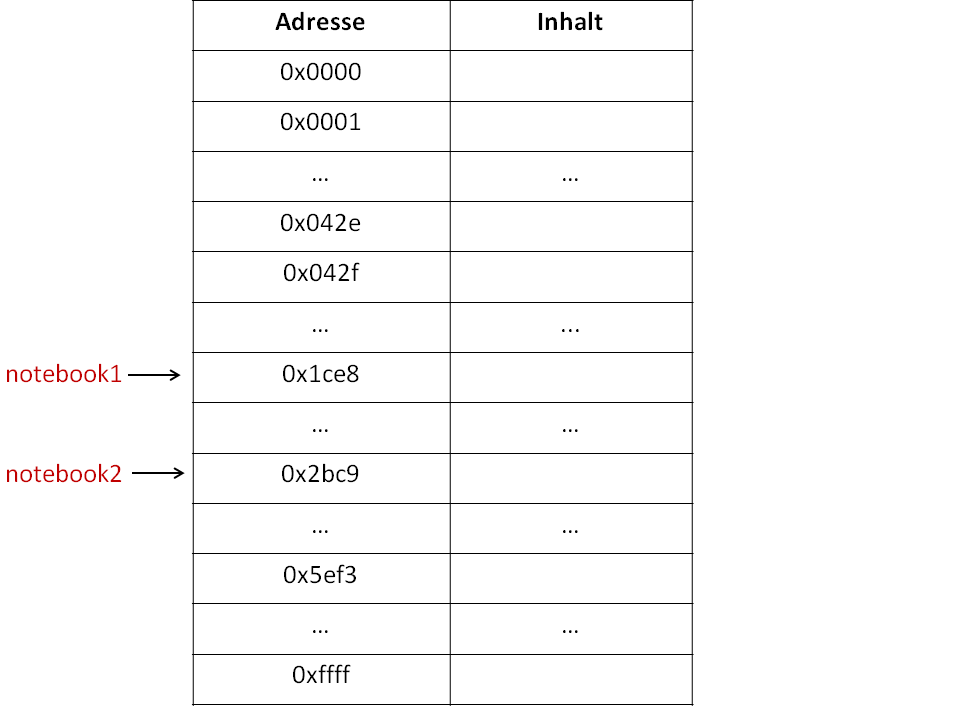
\includegraphics[width=9cm]{logos/deklaration}
\end{frame}

\begin{frame}{Was ist hier passiert?}
2. Objekte wurden mit \textbf{new} erzeugt:\\ 
  \ \\ 
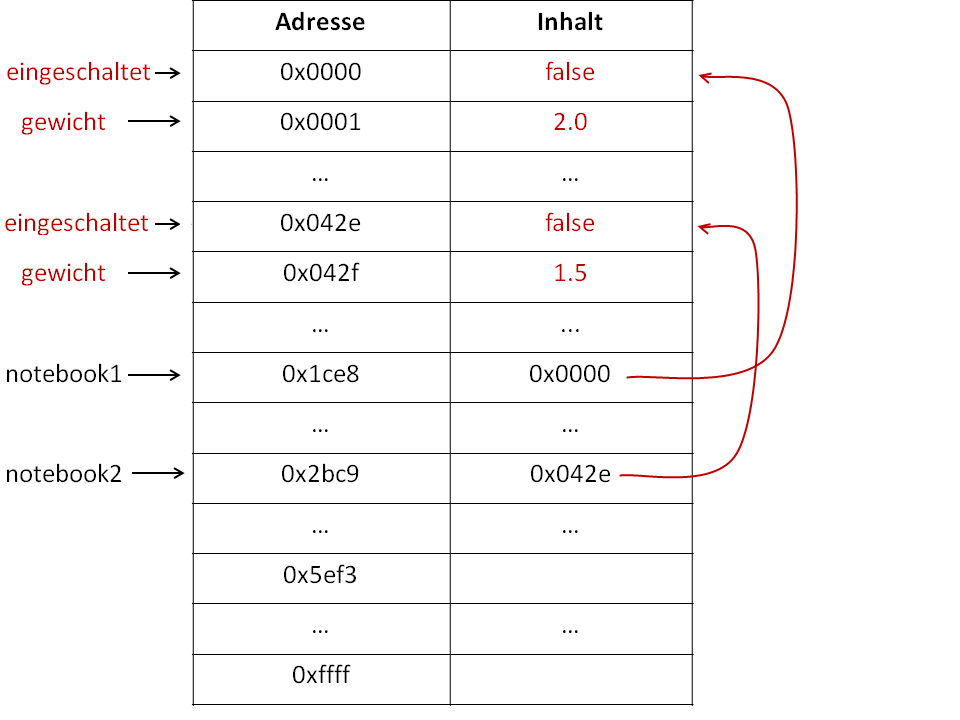
\includegraphics[width=9cm]{logos/erzeugung}
\end{frame}

\begin{frame}{Was ist hier passiert?}
3. \textbf{notebook3} wurde die Referenz von \textbf{notebook1} zugewiesen:\\
  \  \\ 
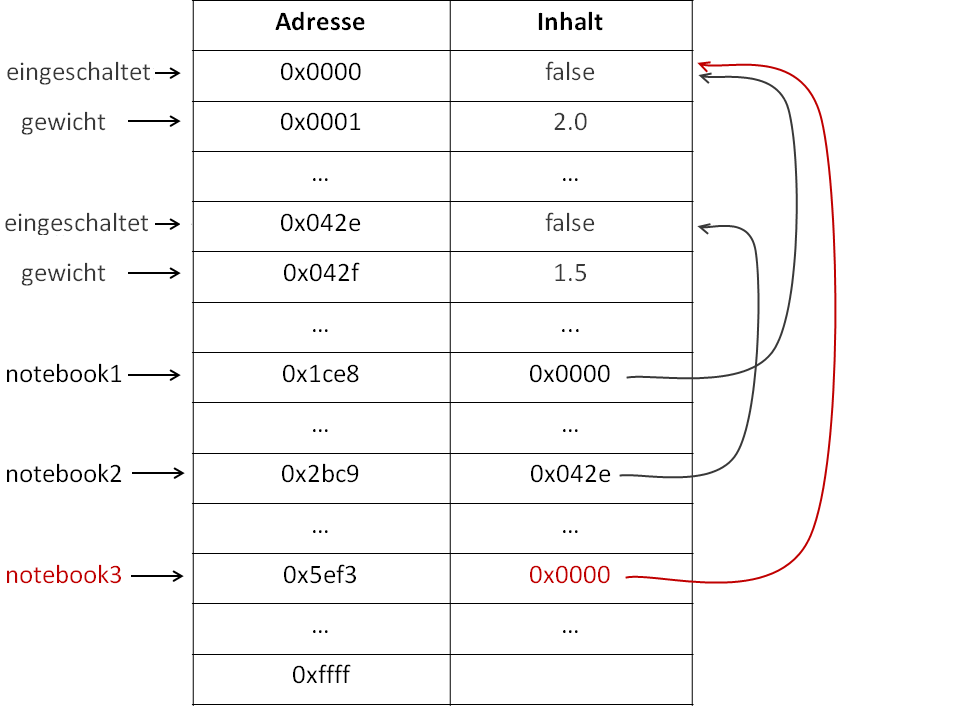
\includegraphics[width=9cm]{logos/notebook3}
\end{frame}

\begin{frame}{Was ist hier passiert?}
4. \textbf{notebook1} \& \textbf{notebook2} wurden eingeschaltet:\\
  \  \\ 
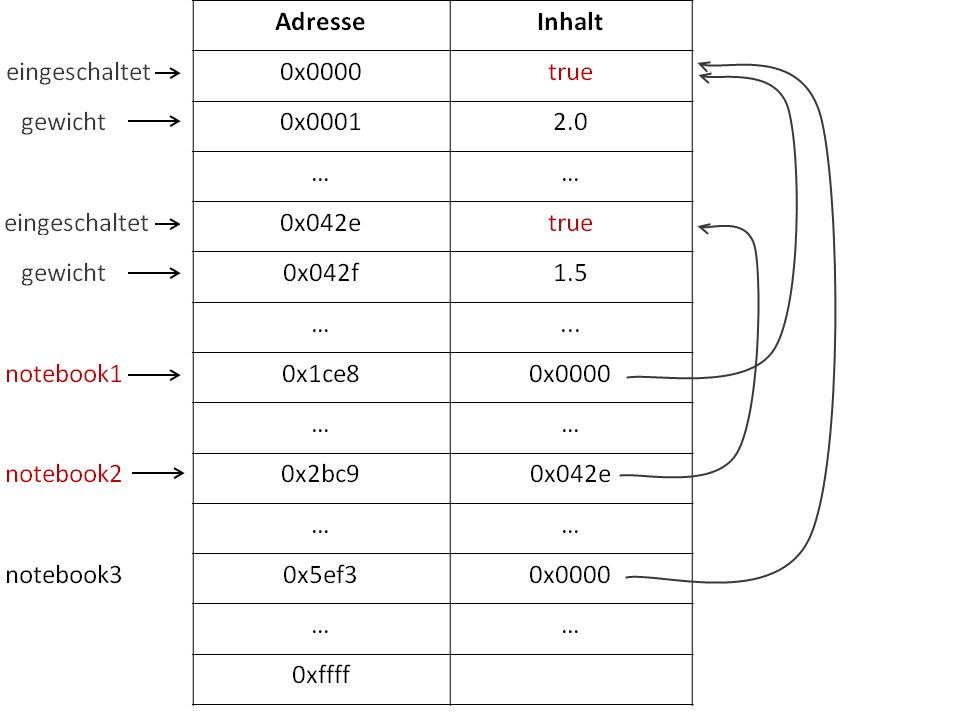
\includegraphics[width=9cm]{logos/eingeschaltet}
\end{frame}

\begin{frame}{Was ist hier passiert?}
5. \textbf{notebook3} (= \textbf{notebook1}) wurde ausgeschaltet:\\
  \  \\ 
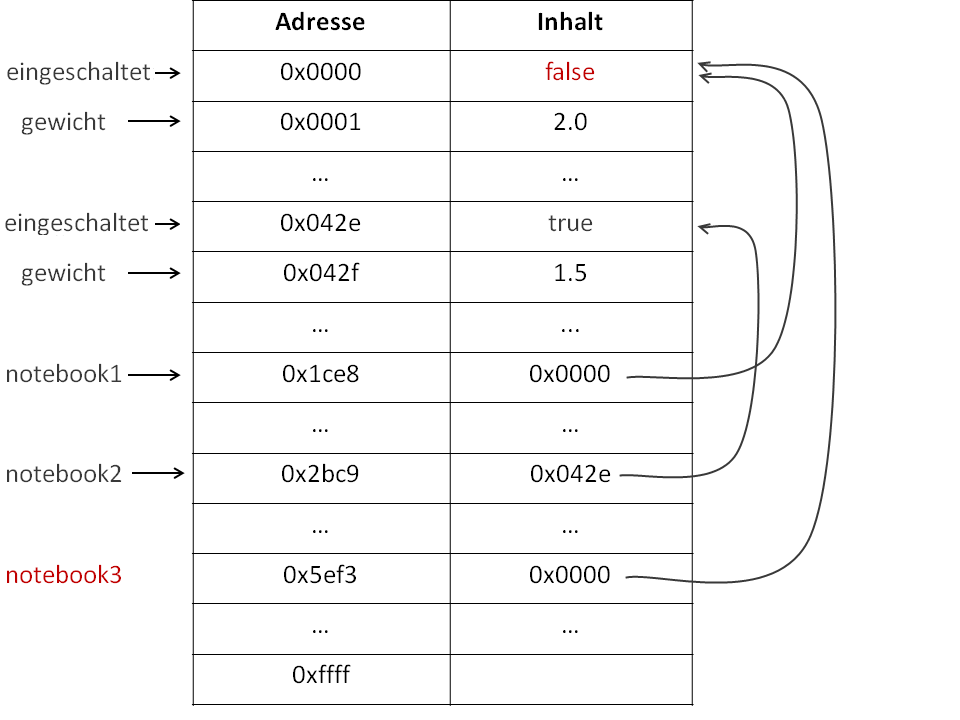
\includegraphics[width=9cm]{logos/ausgeschaltet}
\end{frame}

\begin{frame}{Hinweis:}
\begin{alertblock}{Beachte:}
Anders als bei elementaren Typen wird bei Klassentypen durch den ''='' - Operator nur die \textbf{Referenz} auf das Objekt und nicht das Objekt selbst kopiert!
\end{alertblock}
\pause
\begin{block}{Ausnahme:}
Strings lassen sich durch ''='' kopieren, obwohl String ein Klassentyp ist.
\end{block}
\end{frame}

\section{"Verhalten" modelieren}

\subsection{Methoden}

\begin{frame}{Methoden}
\begin{block}{Was ist eine Methode?}
Eine Methode ist ein Konstrukt, mit dem das \textbf{dynamische Verhalten} von Objekten realisiert wird.
\end{block}
\pause
Mit anderen Worten: Mit Methoden können Objekte endlich etwas ''machen''!
\end{frame}

\begin{frame}[containsverbatim]{Methoden}
\begin{exampleblock}{Beispiel:}
\begin{lstlisting}[basicstyle=\scriptsize]
class Calculator {

	int memValue;			//der Speicher des Taschenrechners

	int add(int x, int y) {
		return x + y;			//gibt die Summe von x und y zurueck
	}

	void memoryWrite(int x) {
		this.memValue = x;		//schreibt den Wert von x in den Speicher
	}

	int memoryRead() {
		return this.memValue;	//gibt den gespeicherten Wert zurueck
	}

	void memoryReset() {
		this.memValue = 0;		//setzt den Speicher auf 0 zurueck
	}
}
\end{lstlisting}
\end{exampleblock}
\end{frame}

\begin{frame}{Methoden}
\begin{block}{Allgemein:}
\begin{itemize}
	\item \textit{Rückgabetyp Methodenname} (\textit{Parameter}) \{ \textit{Methodenrumpf} \}
	\item Ergebnisrückgabe mit \textbf{return} \textit{Wert/Variable};
	\item Methoden ohne Rückgabewert haben den ''Rückgabetyp'' \textbf{void}
\end{itemize}
\end{block}
\end{frame}

\begin{frame}[containsverbatim]{Wie benutzt man nun den Taschenrechner?}
\begin{exampleblock}{Beispiel:}
\begin{lstlisting}[basicstyle=\scriptsize]
class CalculatorTest {
	
	public static void main(String[] args) {
		Calculator myCalc = new Calculator();	//einen Taschenrechner 
												//erzeugen
		int sum = myCalc.add(17, 12);			//etwas addieren
		System.out.println("17 + 12 = " + sum);	//und ausgeben
		myCalc.memoryWrite(42);					//den Speicher beschreiben
		System.out.println(myCalc.memoryRead());//auslesen
		myCalc.memoryReset();					//und loeschen
		System.out.println(myCalc.memoryRead());//testen, ob wirklich 
												//geloescht
	}
}
\end{lstlisting}
\end{exampleblock}
\pause
$\Rightarrow$ alle Klassen kompilieren \& Programm mit ''java CalculatorTest'' ausführen!
\end{frame}

\begin{frame}{Programme ausführbar machen}
\begin{block}{Allgemein}
\begin{itemize}
	\item In einer (separaten) Klasse eine \textbf{main-Methode} schreiben:\\
		public static void main(String[] args) \{...\}
\end{itemize}
\end{block}
\end{frame}

\section{Code Conventions}
\begin{frame}{Code Conventions}
        \begin{block}{Warum?}
                \begin{itemize}
                        \item Code wesentlich leichter zu lesen, übersichtlicher, schöner
                        \item leichteres Einarbeiten in Projekte (Teamarbeit)
                        \item Jeder versteht den code (nicht nur du selbst!)
                        \item Man versteht den code selbst besser!
                \end{itemize}
        \end{block}
        Code Conventions für Java von Oracle:\\
        \url{http://www.oracle.com/technetwork/java/codeconventions-150003.pdf}
\end{frame}

\begin{frame}[fragile]{Code Conventions}
        \begin{block}{Zeilenbreite}
                Zeilen sollten nicht länger als 120 Zeichen sein
        \end{block}
        \begin{block}{Kommentare}
                \begin{itemize}
                        \item sehr nützlich um Code verständlich zu machen
                        \item wichtiges Werkzeug für Dokumentation (javadoc)
                \end{itemize}
                \begin{lstlisting}[basicstyle=\scriptsize]
                // gibt die Anzahl Studenten an
                int studentCount;
                
                /* es gibt in Java
                 auch mehrzeilige
                 Kommentare */
                \end{lstlisting}
        \end{block}
\end{frame}

\begin{frame}[fragile]{Code Conventions}
        \begin{block}{Eine Deklaration pro Zeile, gleicher Datentyp}
                \begin{lstlisting}[basicstyle=\scriptsize]
                /* guter Stil: */                
                int studentCount; // gibt die Anzahl der Studenten an
                int tutorCount; // gibt die Anzahl der Tutoren an
                
                /* schlechter Stil: */
                int studentCount, tutorCount;
                
                /* noch schlimmer: */
                int x, y, z[];
                \end{lstlisting}
        \end{block}
\end{frame}

\begin{frame}[fragile]{Code Conventions}
        \begin{block}{Variablen vor Blocks deklarieren}
                \begin{itemize}
                        \item Variablen sollten so früh wie möglich deklariert werden
                        \item Nicht erst dann, wenn sie benötigt werden (Ausnahme: for-Schleife)
                \end{itemize}
                \begin{lstlisting}[basicstyle=\scriptsize]
                // Beispiel:
                public void myMethod() {
                 int x;
                        
                 if(condition) {
                 int y;
                 ...
                 }
                }
                \end{lstlisting}
        \end{block}
\end{frame}

\begin{frame}[fragile]{Code Conventions}
        \begin{block}{Klassen, Interfaces und Funktionen sauber formatieren}
                \begin{itemize}
                        \item Kein Leerzeichen zwischen Methodenname und "("
                        \item \{ in der gleichen Zeile wie Klassen/Methodenname
                        \item \} in einer eigenen Zeile am Ende
                        \item Methodennamen mit freier Zeile trennen
                \end{itemize}
                \begin{lstlisting}[basicstyle=\scriptsize]
                class Sample extends Object {
                 int ivar1;
                 int ivar2;
                
                 Sample(int i, int j) {
                 ivar1 = i;
                 ivar2 = j;
                 }
                
                 int emptyMethod() { }
                
                 ...
                }
                \end{lstlisting}
        \end{block}
\end{frame}

\begin{frame}[fragile]{Code Conventions}
        \begin{block}{Leerzeichen bei Operatoren setzen}
         \begin{itemize}
         \item sieht einfach besser aus und ist übersichtlicher!
         \end{itemize}
                \begin{lstlisting}[basicstyle=\scriptsize]
// unerwuenscht:
int x=42;
int y=(x-32)*10+9;
                
// besser:
int x = 42;
int y = (x - 32) * 10 + 9;
                \end{lstlisting}
        \end{block}
\end{frame}

\begin{frame}[fragile]{Code Conventions}
        \begin{block}{Naming Conventions}
         \begin{itemize}
         \item \url{Klassen} sollten Substantive sein, beginnend mit Großbuchstaben
         \item[] \lstinline$class ImageSprite { ... }$
         \item \url{Methoden} sollten Verben sein, beginnend mit Kleinbuchstaben
         \item[] \lstinline$private int getCount();$
         \item \url{Variablen} beginnen mit Kleinbuchstaben, kurz aber aussagekräftig
         \item[] \lstinline$int imageWidth;$
         \item \url{Konstanten}: jeder Buchstabe groß, Wörter getrennt durch Underscore
         \item[] \lstinline$public static final int MAX_WIDTH = 800$
         \end{itemize}
        \end{block}
\end{frame}

\begin{frame}[fragile]{Code Conventions}
        \begin{figure}[ht]
        \centering
      \includegraphics[width=0.8\textwidth]{camelcase.png}
    \end{figure}
\end{frame}

\begin{frame}
Tutoriumsaufgabe
\end{frame}

\section{Zum Übungsblatt 1}
\subsection{Hinweise}

\begin{frame}{Hinweise zum Übungsblatt}
\begin{itemize}
\item Ausgabe online im Praktomat oder auf Vorlesungsseite

\item Abgabetermin: Montag, der 11. November 2013, 13 Uhr

\item Abgabe online im Praktomaten $ \Rightarrow $ Uni-Netz oder VPN erforderlich

\item keine Bibliotheken verwenden, die im Übungsblatt nicht explizit zugelassen wurden (z.B. kein "Date")

\item keine ungewollte Funktionalität einbauen – es gilt die Devise:\\ Einfache Fragen erfordern einfache Antworten!}
\end{itemize}
\end{frame}

\section{Hinweise zum Praktomat}
\begin{frame}{Praktomat}
\begin{itemize}
\item \textbf{Hat sich jeder im Praktomat angemeldet?}
\item Abgabe \textbf{NUR} im Praktomat.

\item Abgabe immer Montags bis 13 Uhr.

\item Der Praktomat spinnt manchmal etwas, also immer so früh wie möglich probieren abzugeben!

\item Für das erste Blatt überprüft der Praktomat nur die Zeilenbreite: Maximal 120 Zeichen!

\item In Zukunft wird auch Übersetzbarkeit mit javac geprüft.
\end{itemize}
\end{frame}

\begin{frame}{Erinnerungen}
\begin{alertblock}{Warnung!}
\begin{itemize}
\item \emph{\f{Nicht abschreiben!}}

\item Schon bei \textbf{einmaligem} Nachweis verwirkt man die Chance auf den Übungsschein!

\item Ohne Schein darf man die Abschlussaufgabe nicht schreiben!

\item Nur mit beidem besteht man das Modul Programmieren!

\item Programmieren ist Teil der Orientierungsprüfung!

\item Ohne bestandene Orientierungsprüfung bis zum 3. Semester fällt man aus dem Studium und darf bundesweit das Studienfach nicht mehr belegen.
\end{itemize}
\end{alertblock}
\end{frame}


\begin{frame}{Ende}
	\begin{center}
	\huge{Vielen Dank für die Aufmerksamkeit!}
	\normalsize Habt ihr noch Fragen?
	\end{center}
\end{frame}

\appendix
\beginbackup

%\begin{frame}[allowframebreaks]{References}
%	\printbibliography
%\end{frame}

\backupend

\end{document}
